\subsection{Interface model}

The user interface provides a convenient way to interact with the functional model to display and modify data. The user interface offers a consistent design, which runs through the entire system.

\subsubsection{Product view}

\begin{wrapfigure}{r}{0.5\textwidth}
    \centering
    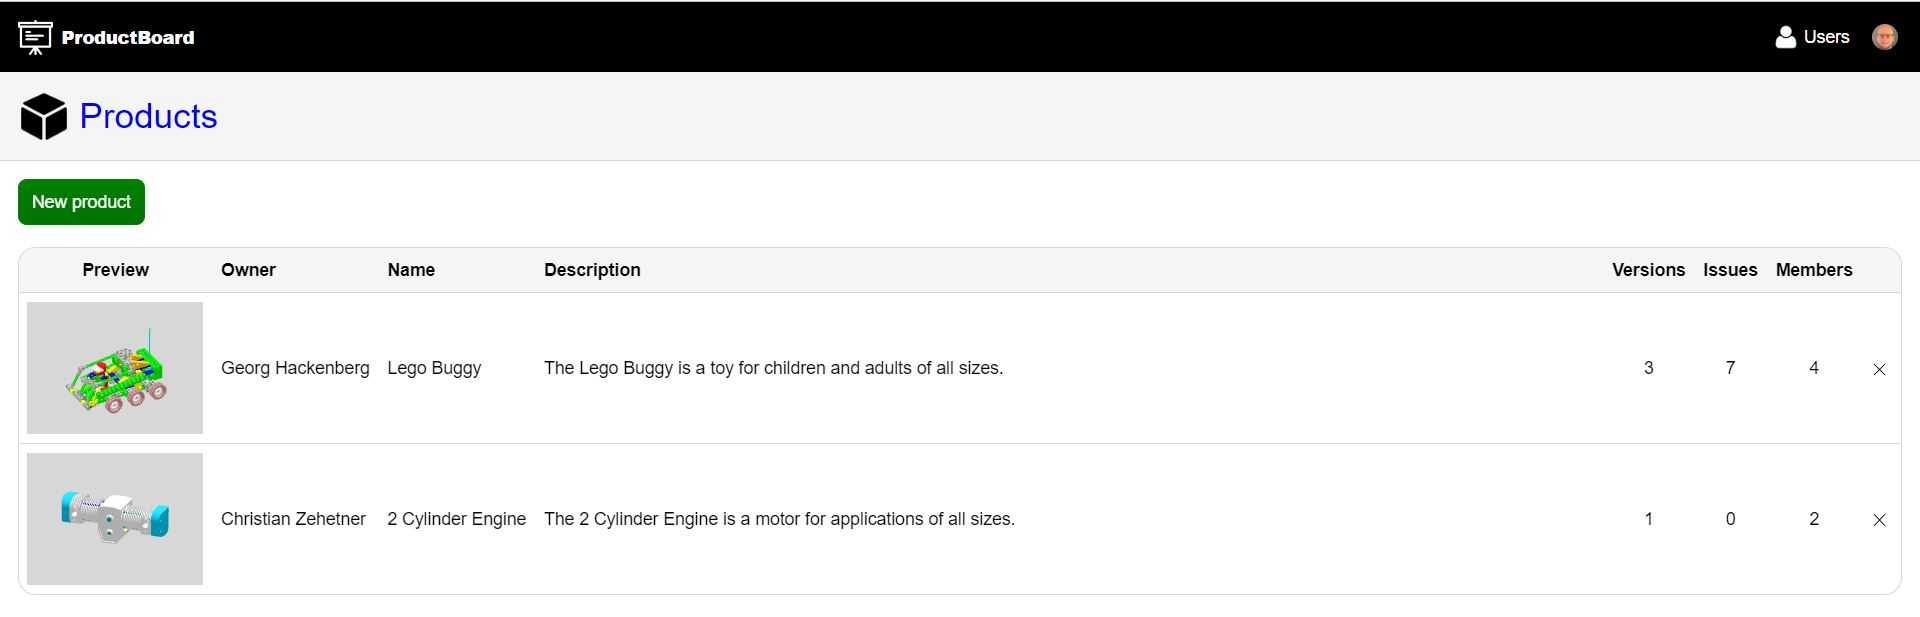
\includegraphics[width=0.5\textwidth]{startpage.JPG}
    \caption{Product view}
    \label{fig: startpage}
\end{wrapfigure}

The \textit{product view} page lists all available products, for which the user has the permission to see them, in a table [see Fig. \ref{fig: startpage}]. For each product in the table a preview is shown. The other columns show the attributes \textit{owner, name, description, versions, issues and members}. The X on the right provides the possibility to delete the corresponding product. The owner is the person who created the product. Name and description are defined when the product is created and can be changed later. The columns on the right show how many versions exist for this product, how many issues have been created and how many members have access to the product. By clicking on New product you get also to the ProductSettings view where you can add a new product when you have the product management permission. This button is only visible when the corresponding user has product management permission. The CAD model and version details will be added when the user creates a new version of a product.

\subsubsection{ProductVersion view}

\begin{wrapfigure}{r}{0.5\textwidth}
    \centering
    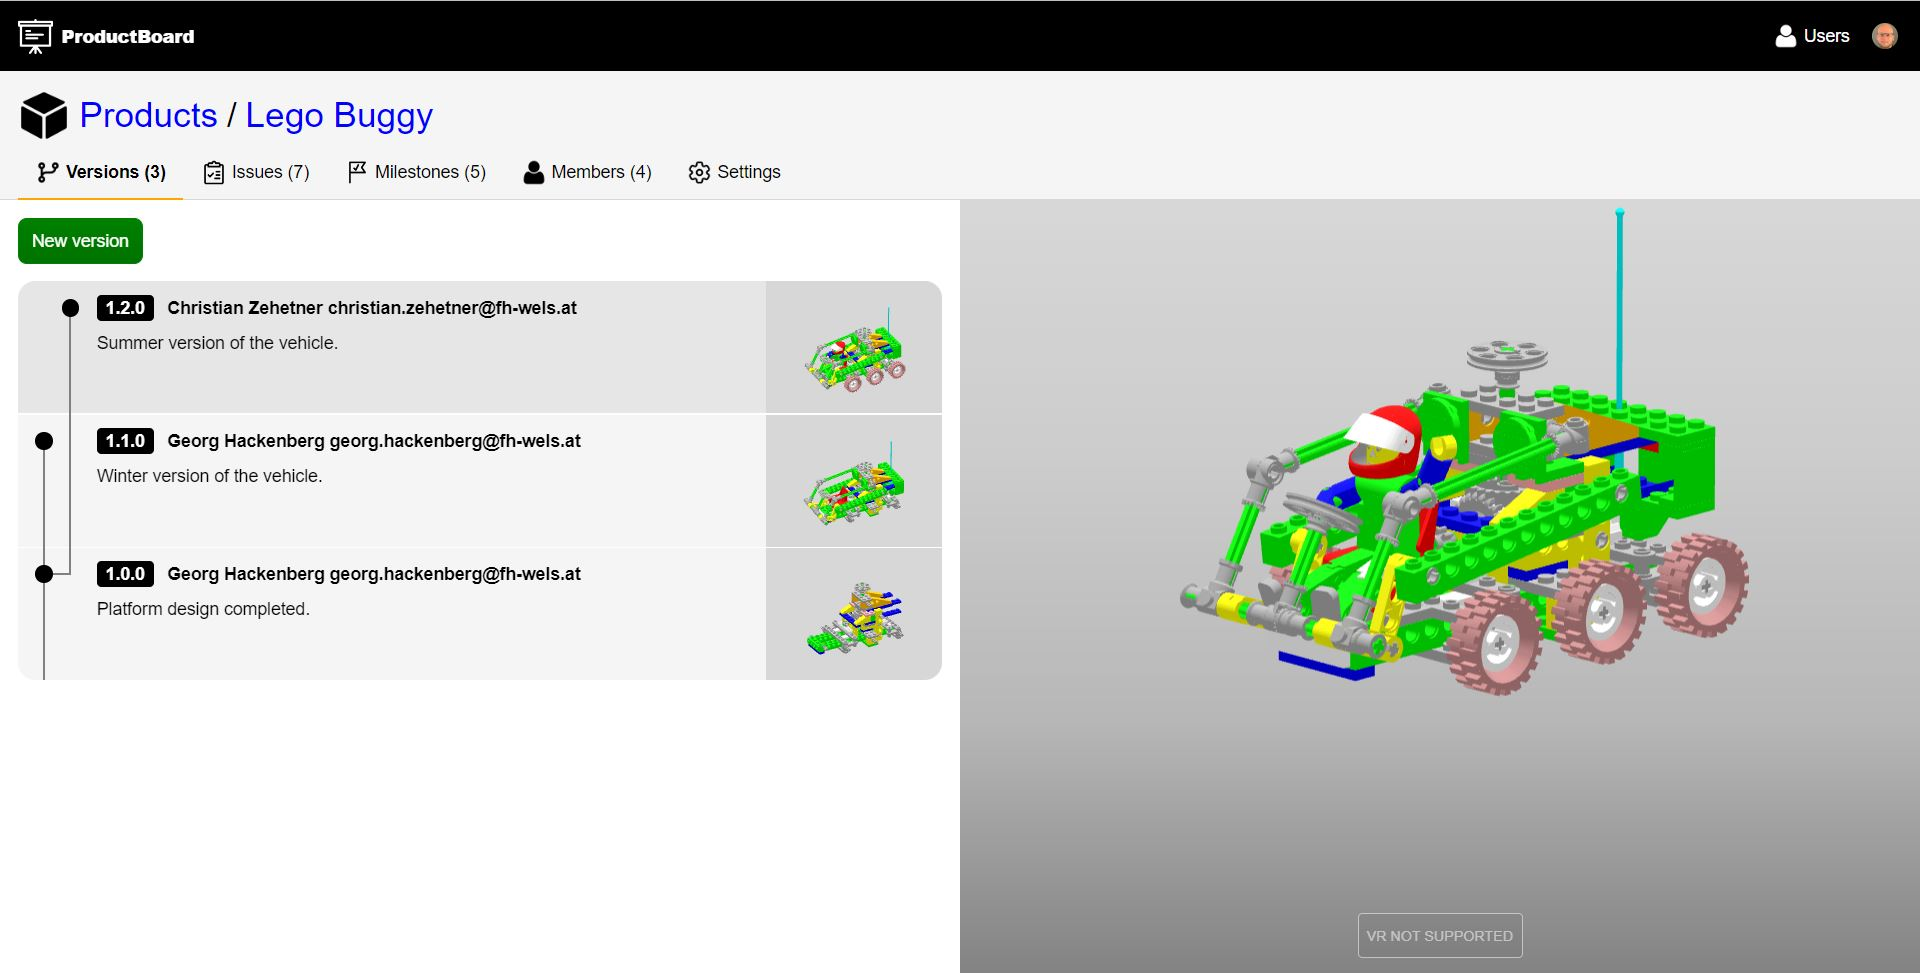
\includegraphics[width=0.5\textwidth]{versionview.JPG}
    \caption{ProductVersion view}
    \label{fig: versionview}
\end{wrapfigure}

Clicking on a product takes you to the ProductVersion view. You can also use the toolbar to jump to other pages such as issues, milestones members or settings. The left side of the view shows the created versions. On the left side there is a tree structure similar to GitHub. This tree structure results from the chronological arrangement of the product versions. The lines of the structure show how the product versions are in relation to the respective base versions. In the middle is the corresponding version number with the owner of the version inclusive email and a short description. Each version offers a preview. By clicking on the respective version, the 3D view on the right side also changes and shows the selected model. The 3D view allows to rotate, move and zoom the model. 
With a click on the \textit{New version} button you get to the ProductVersionSettings view where you can create new product versions. [see Fig. \ref{fig: versionview}]. 

\subsubsection{ProductVersionSettings view}

\begin{wrapfigure}{r}{0.5\textwidth}
    \centering
    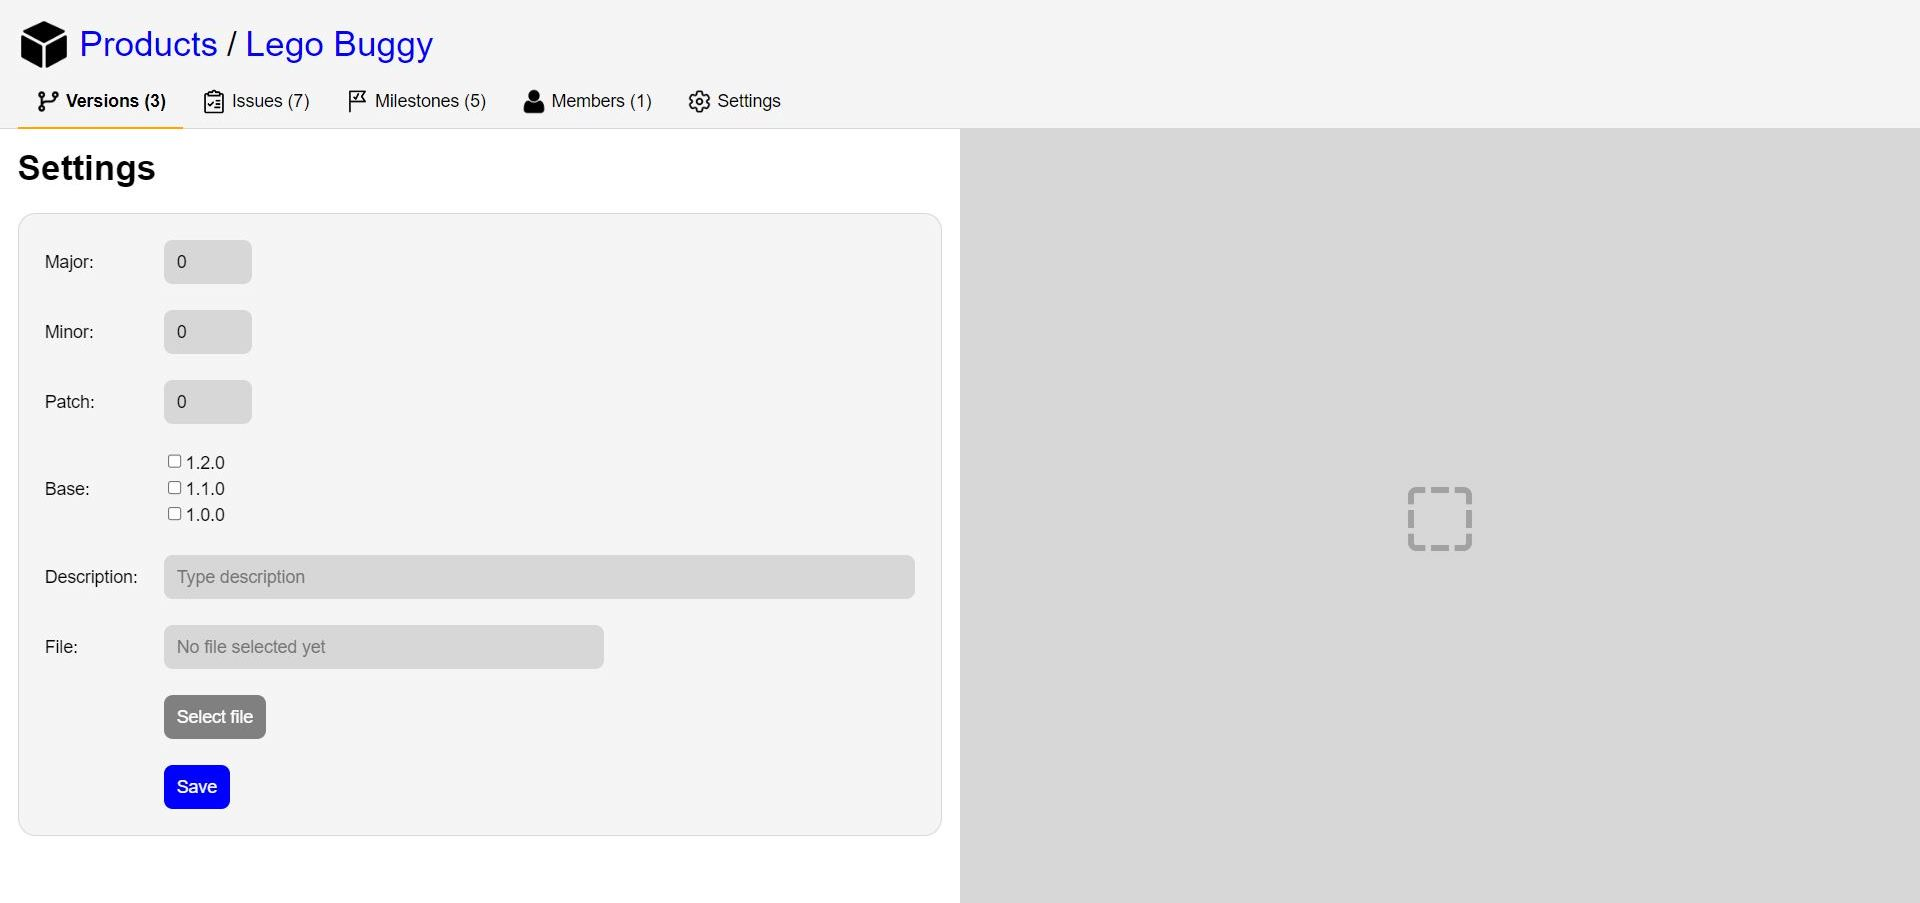
\includegraphics[width=0.5\textwidth]{versionsettingsview.JPG}
    \caption{ProductVersionSettings view}
    \label{fig: versionsettingsview}
\end{wrapfigure}

Here you can enter information for a new version and select an GLB file. Depending on the selected base versions, the ProductVersion view shows the new version with the corresponding new tree structure after pressing the Save button. It is also possible to select multible base versions to merge them into a new version.

\subsubsection{ProductIssue view}

\begin{wrapfigure}{r}{0.5\textwidth}
    \centering
    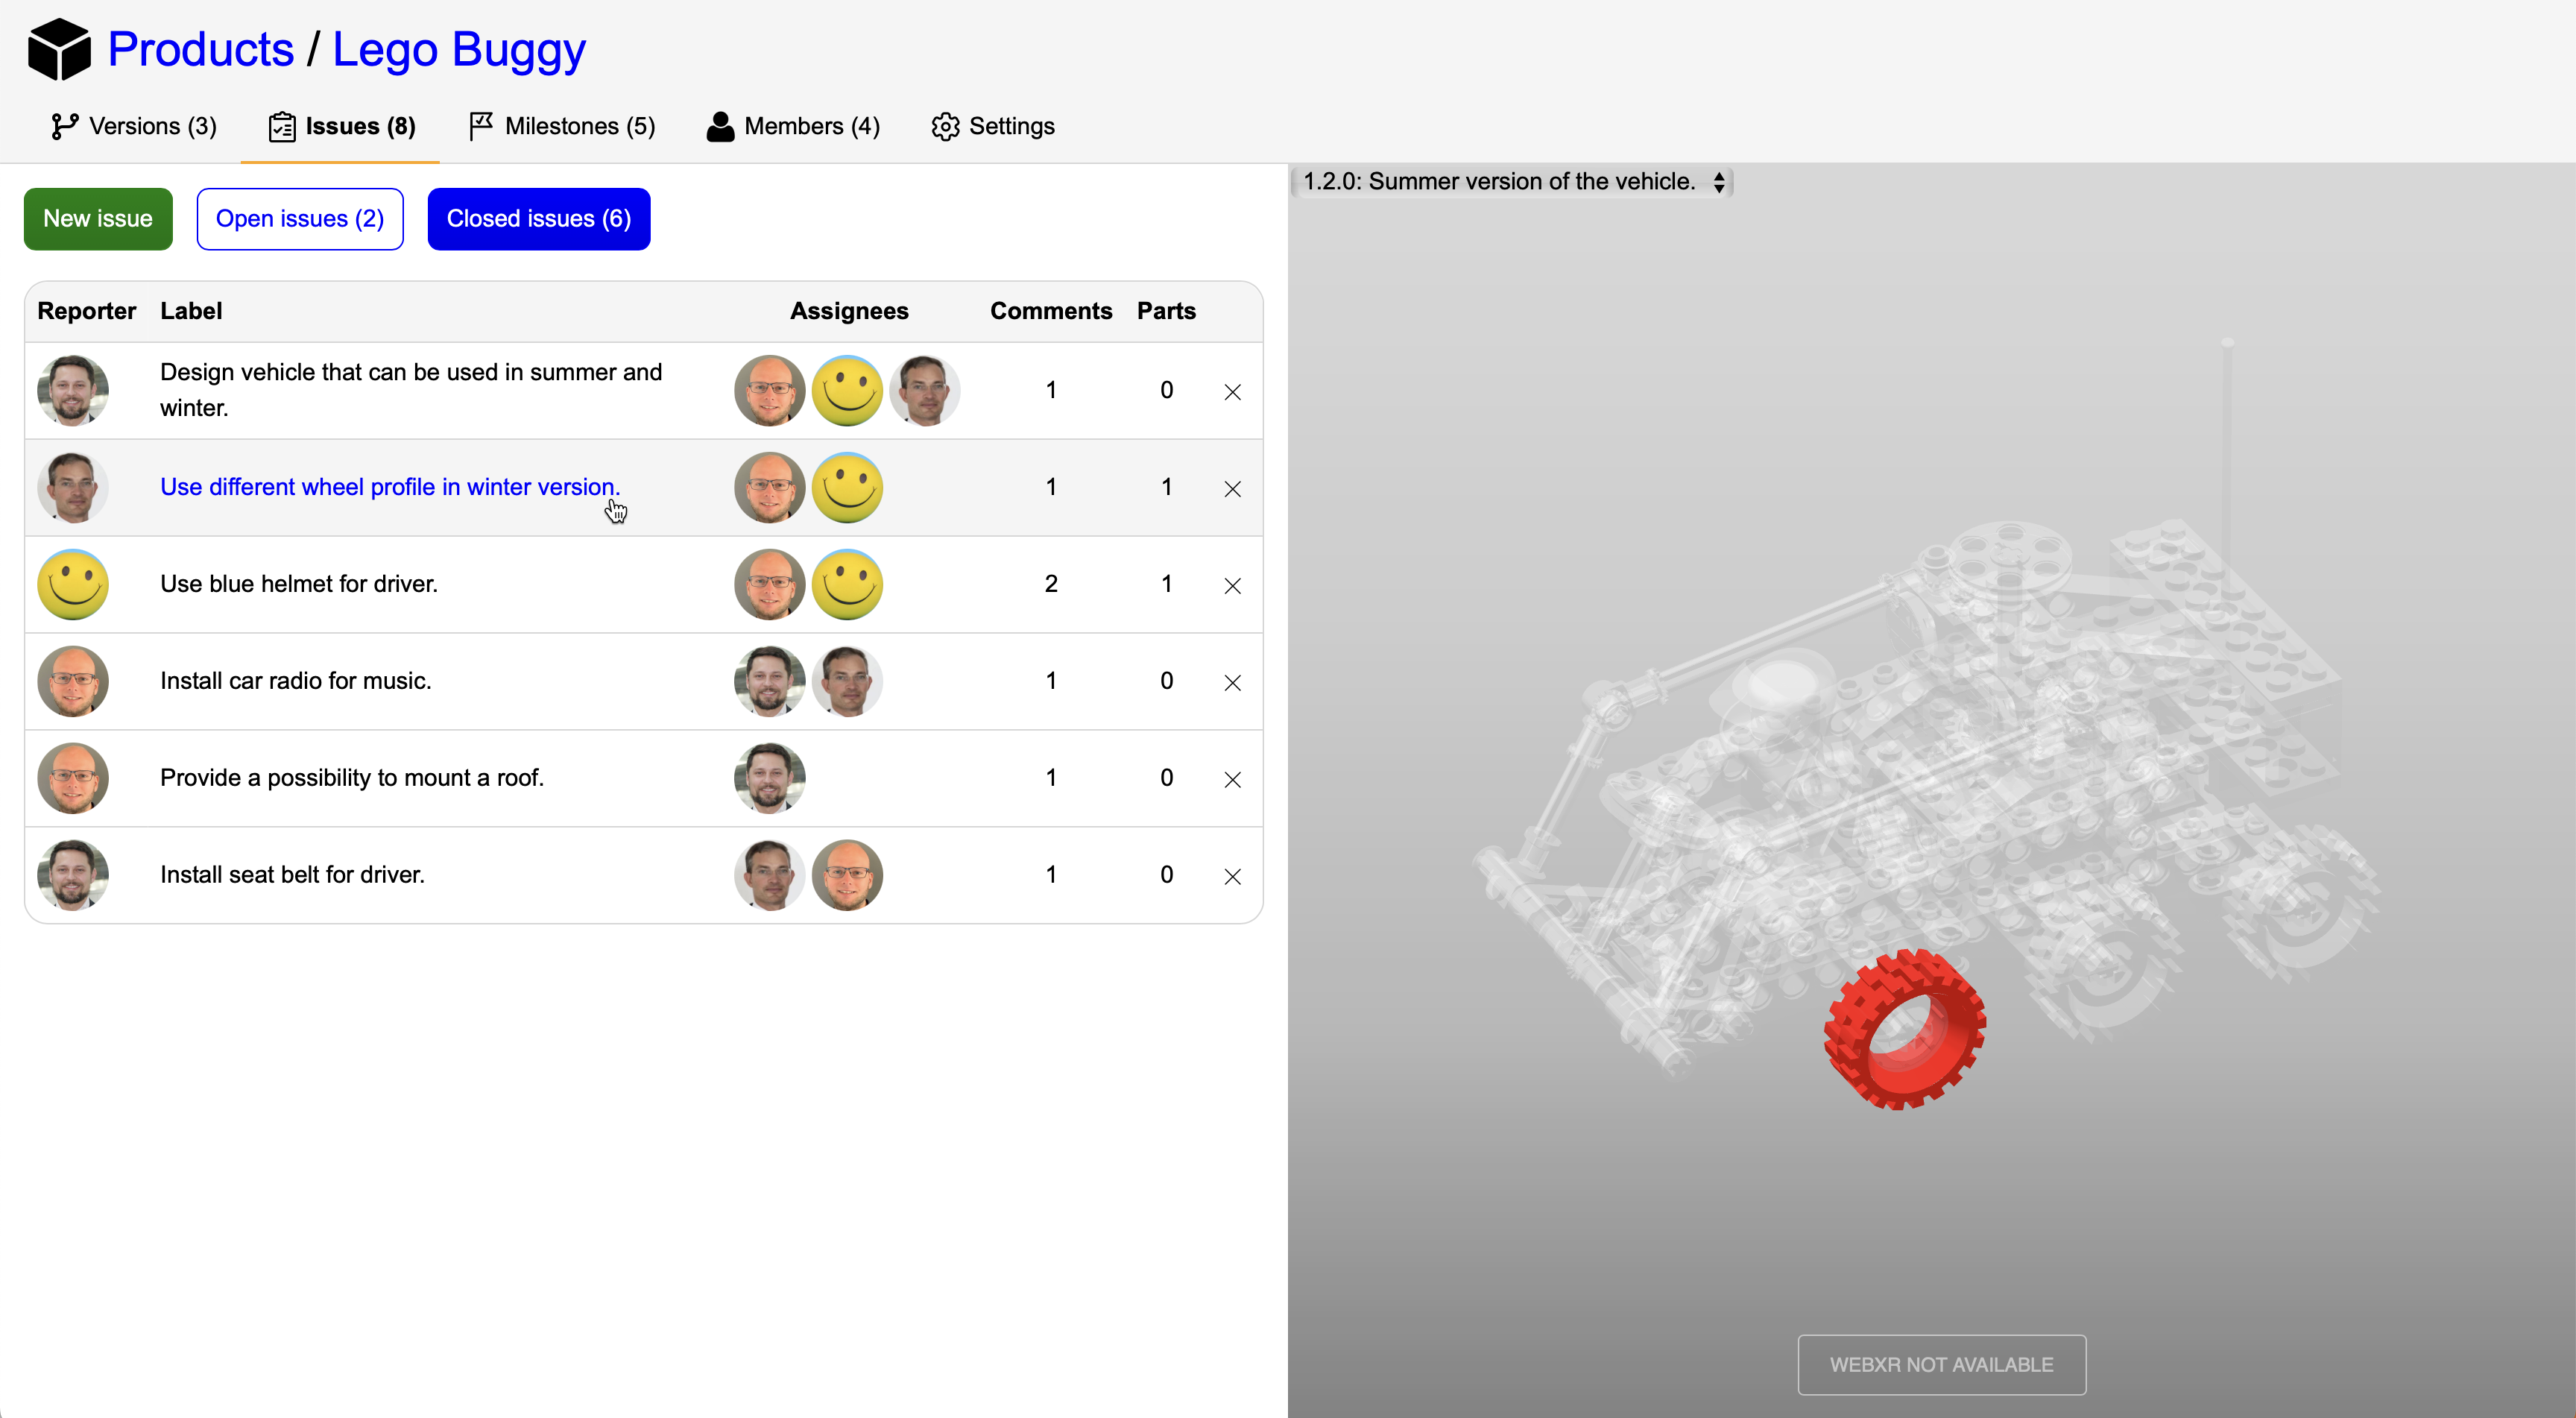
\includegraphics[width=0.5\textwidth]{issueviewselectedpart.png}
    \caption{Issue view}
    \label{fig: issueview}
\end{wrapfigure}

By clicking on the Issues link, you access the ProductIssue view [see Fig. \ref{fig: issueview}]. Here the created issues are displayed in a table. The two buttons Open Issues and Closed Issues can be used to filter the list accordingly. The table shows the reporter who created the issue, the associated label, the assignees and how many comments and marked parts are in the conversation channel. 
All views with 3D View offer the possibility to select a desired version for viewing. In the version view the version can be clicked directly. In the other views the version can be selected via a dropdown menu. This menu is located in the upper left corner of the 3D View. 
If the user hovers with the mouse over a part of the 3D model, this part gets highlighted. 
When hovering over an issue, the 3D view shows those parts that have been referenced in the comments of the respective issue by highlighting them in red.
When hovering over an issue the parts are only highlighted if the version on which the parts were selected was picked in the dropdown menu. Thats because the 3d view shows for each version only the markers that were created on corresponding version.

\subsubsection{ProductIssueSettings view}

\begin{wrapfigure}{r}{0.5\textwidth}
    \centering
    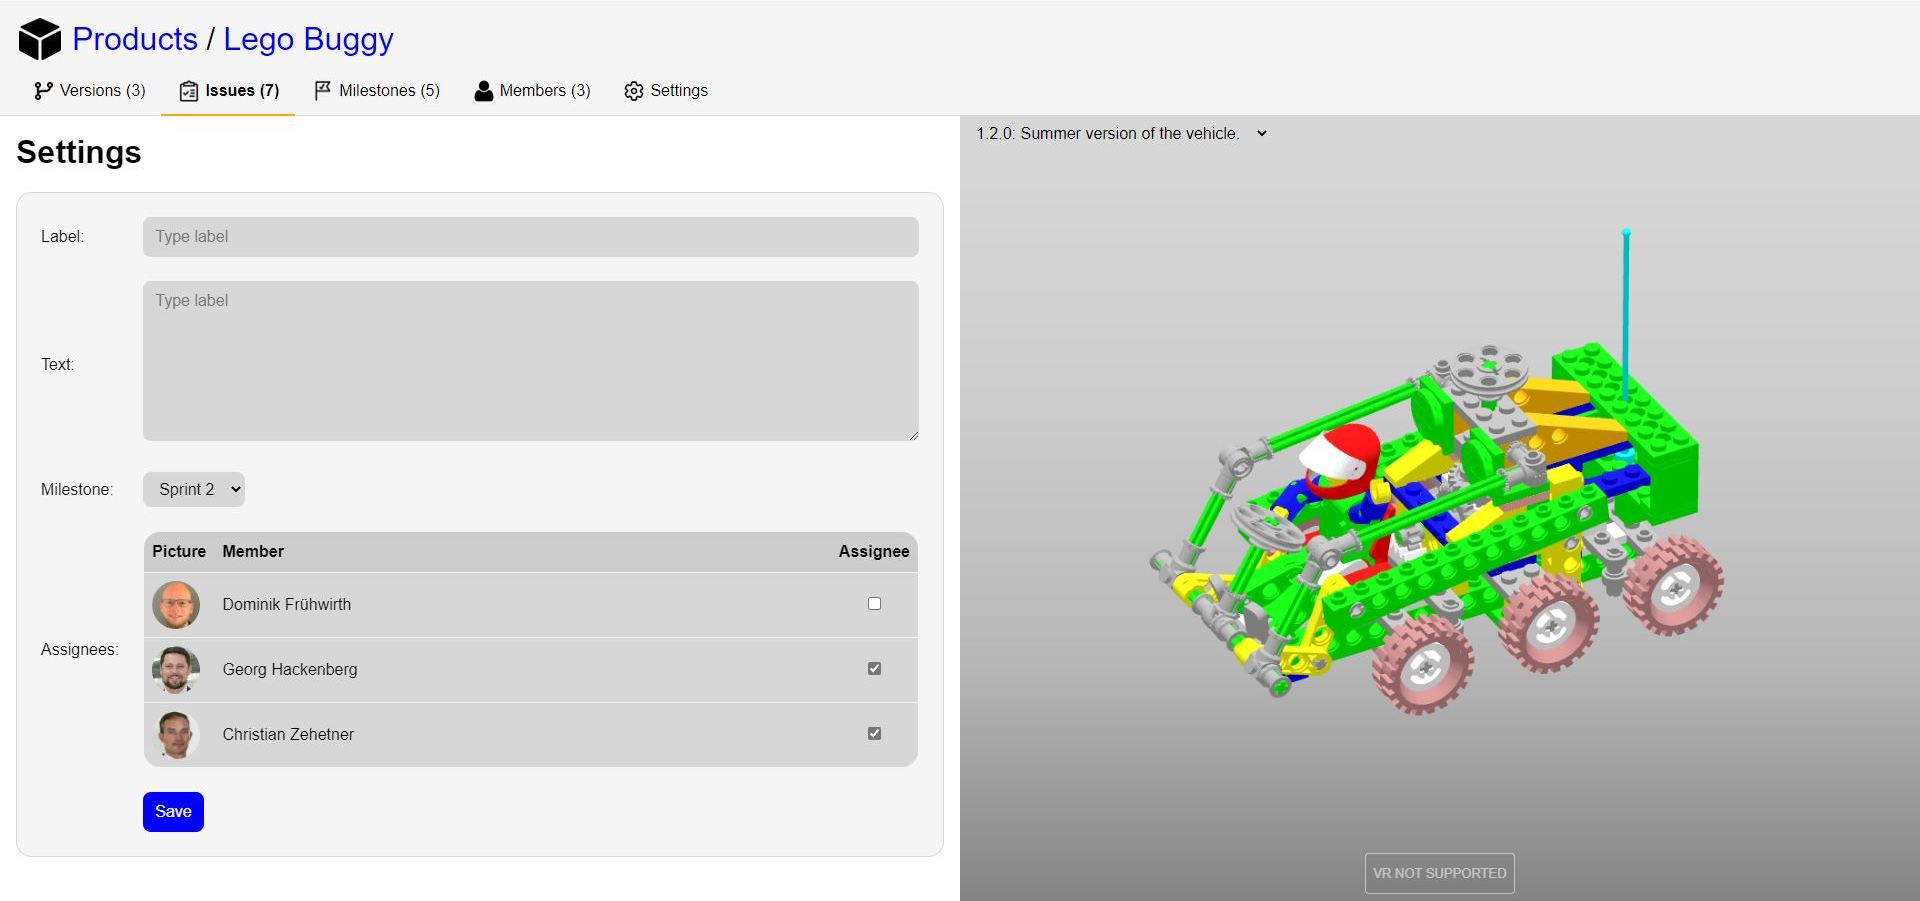
\includegraphics[width=0.5\textwidth]{issuesettingsview.JPG}
    \caption{Issuesettings view}
    \label{fig: issuesettingsview}
\end{wrapfigure}

The ProductIssueSettings view allows to create new issues for the product [see Fig. \ref{fig: issuesettingsview}]. The label, the text, the milestone and the assignees can be defined. An existing milestone can be selected with the dropdown menu. An issue must not be assigned to a milestone. This choice lies by the user. 
As in the ProductIssue view, the model of the desired version can also be selected here via dropdown menu on the 3D view.
The \textit{text} field in the ProductIssueSettings view represents the first comment in an issue. By clicking on the part, the part gets included in the comment as markdown text. If a comment includes a marked part when created, the marking of the respective part is saved to the associated product version.
The Save button closes the settings, and you return to the ProductIssue view where the new issue is visible.

\subsubsection{ProductIssueComment view}

\begin{wrapfigure}{r}{0.5\textwidth}
    \centering
    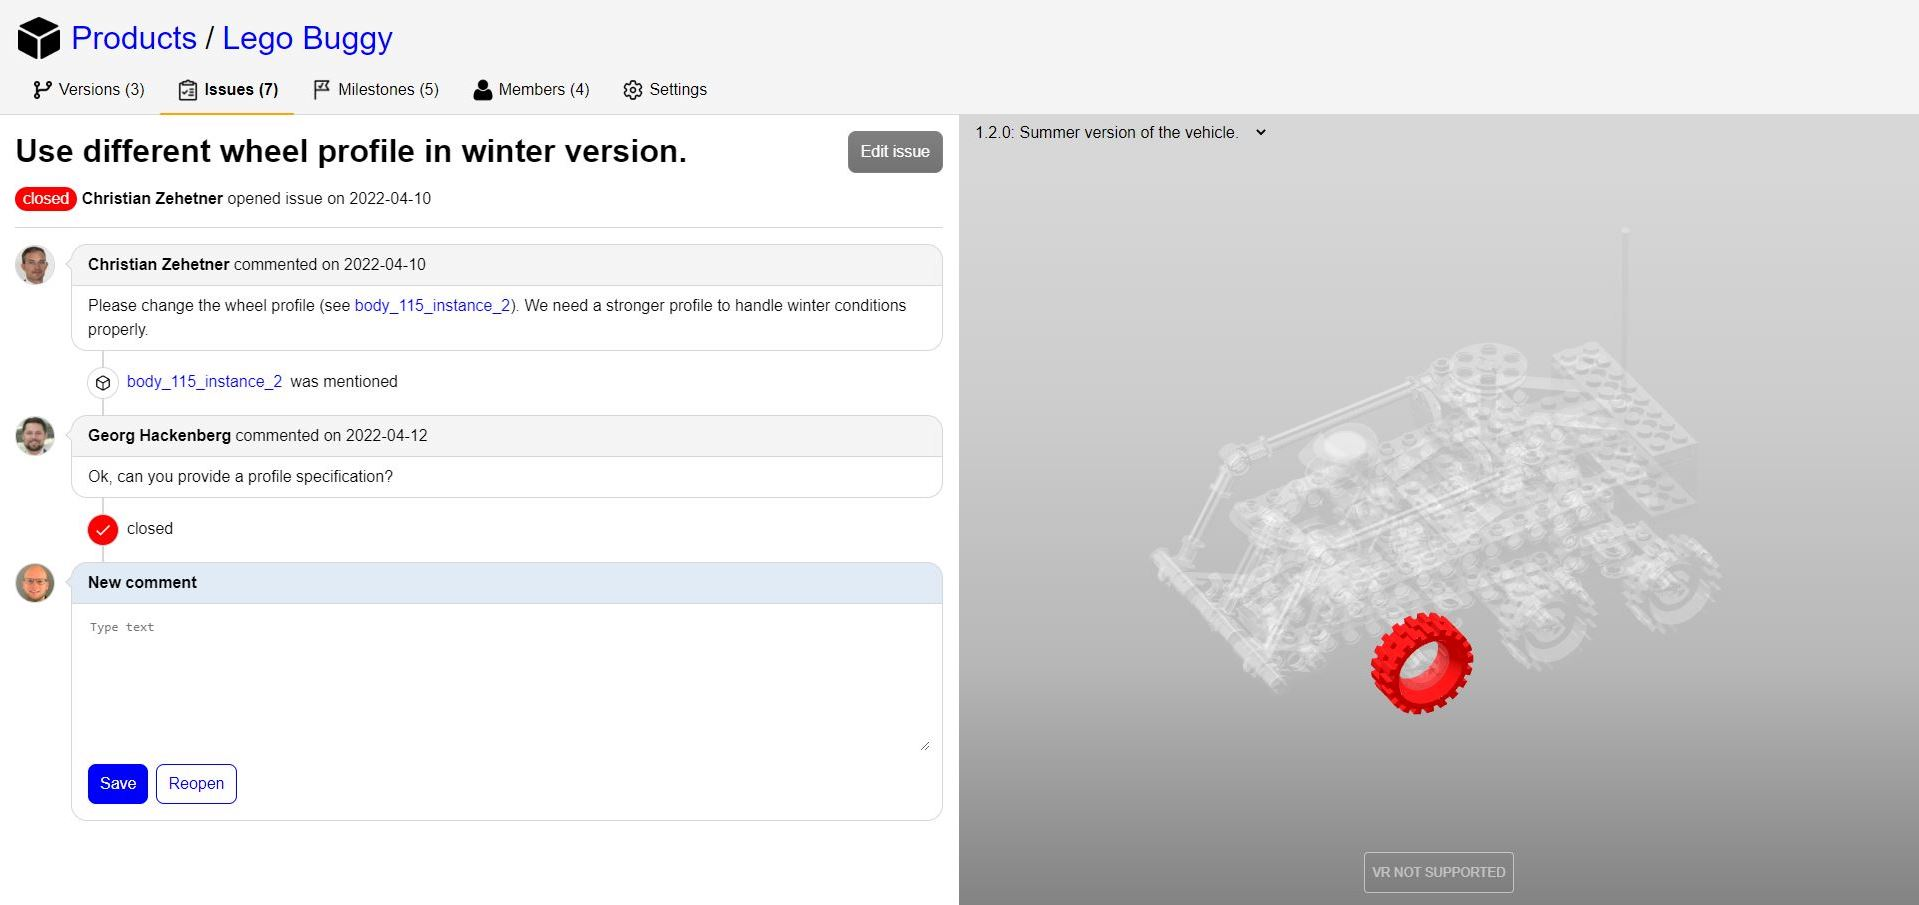
\includegraphics[width=0.5\textwidth]{commentselectedpartview.JPG}
    \caption{Selected part in ProductIssueComment view}
    \label{fig: commentselectedpartview}
\end{wrapfigure}

Clicking on an issue in the Issue view opens the corresponding ProductIssueComment view.  Here you have the possibility to discuss the issue. 
For this purpose, in the new comment box a text can be entered. This text field supports markdown.
Like in the ProductIssueSettings view you can click on a part of the 3D model to mark a part as markdown[see Fig. \ref{fig: commentselectedpartview}]. In the course of a discussion, several parts can be marked in this way.
A comment can also be used to close an issue by clicking the close button. This issue will then be found in Closed Issues in the ProductIssue view. With the comment function it is also possible to reopen the issue in the same way. The Close button displays the text Reopen when an issue is closed. In the upper right corner of the ProductIssueComment view there is a button to edit the selected issue. For example, the issue can be assigned to another Milestone or other attributes like the label, text or the list of assignees can be changed [see Fig. \ref{fig: issuesettingsview}].

\subsubsection{ProductMilestone view}

\begin{wrapfigure}{r}{0.5\textwidth}
    \centering
    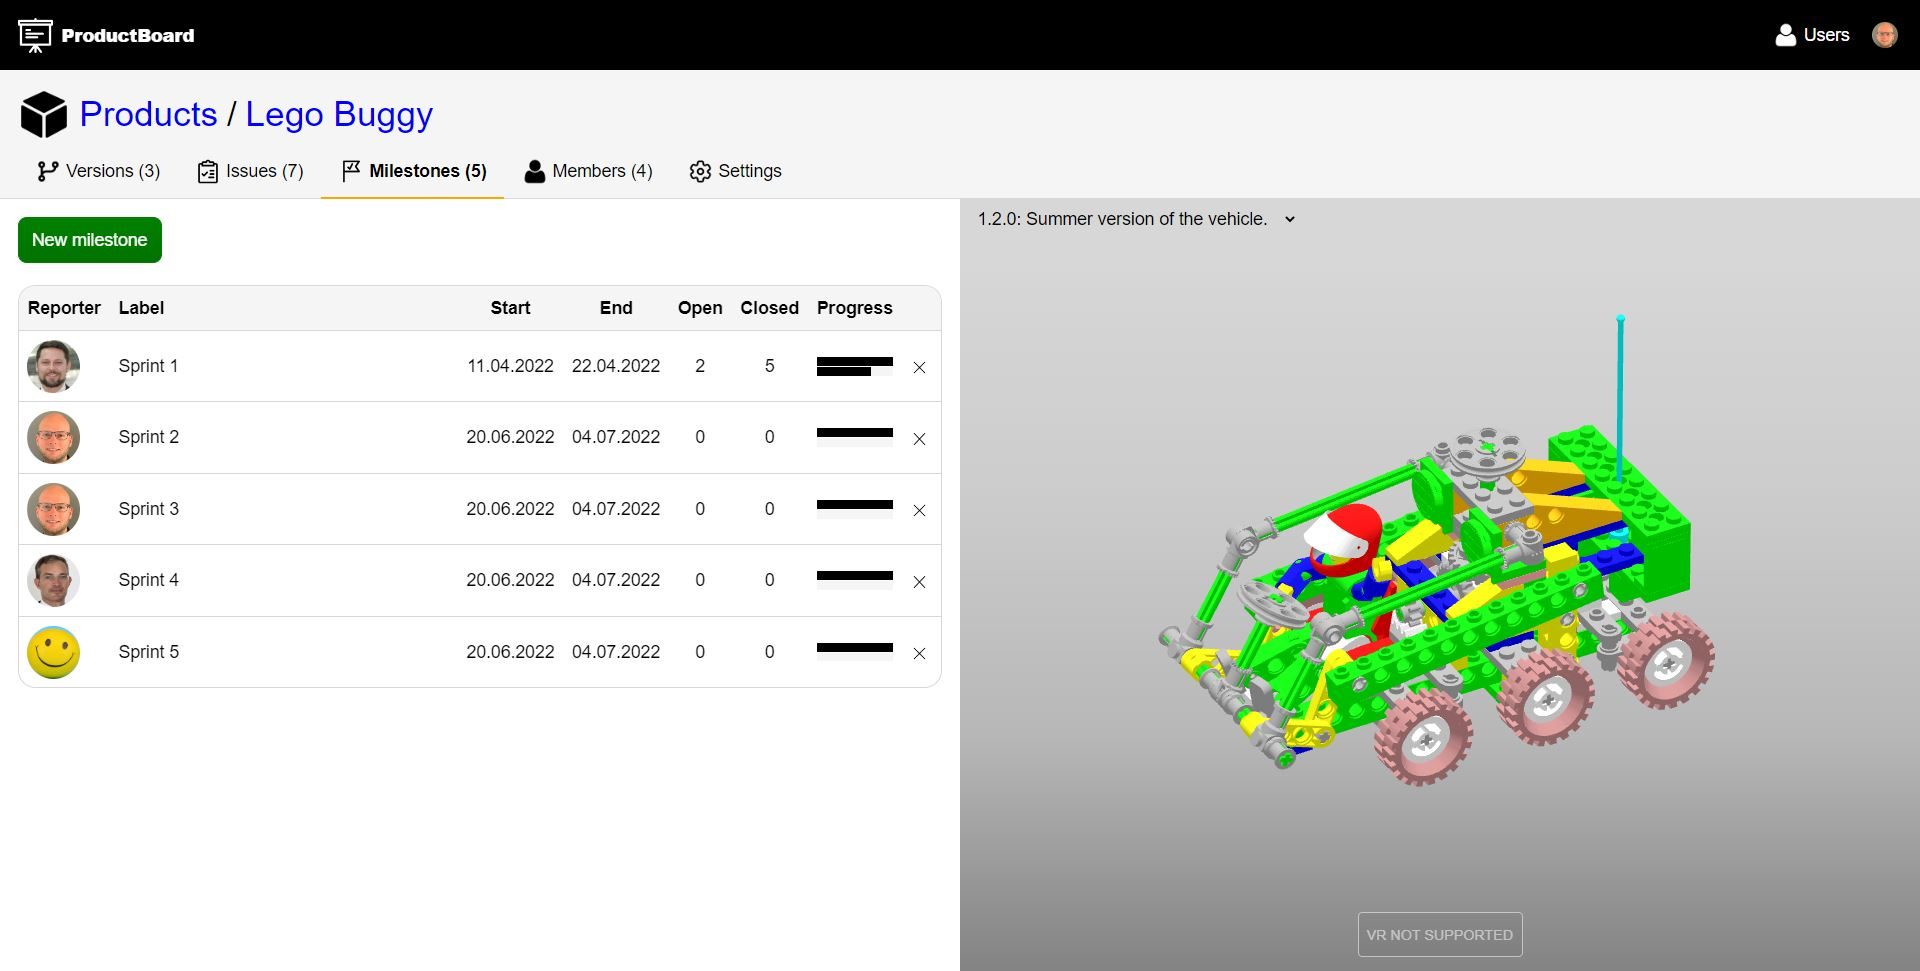
\includegraphics[width=0.5\textwidth]{milestoneview.JPG}
    \caption{ProductMilestone view}
    \label{fig: milestoneview}
\end{wrapfigure}

The ProductMilestone view can be accessed via the Milestones link [see Fig. \ref{fig: milestoneview}]. A table shows who created the milestone, its name, start date, end date and the progress. For each milestone two progress bars are displayed. The first one shows the date progress of a milestone by calculating \textit{100 * (nowDate - startDate) / (endDate - startDate)}. The second bar shows the issue progress of a milestone by calculating \textit{100 * number of closedIssues / number of allIssues}.
A click on the New Milestone button leads to the ProductMilestoneSettings view. Here the attributes of a milestone can be adjusted and saved. The new or edited Milestone than show up in the ProductMilestone view.

\subsubsection{ProductMilestoneIssue view}

\begin{wrapfigure}{r}{0.5\textwidth}
    \centering
    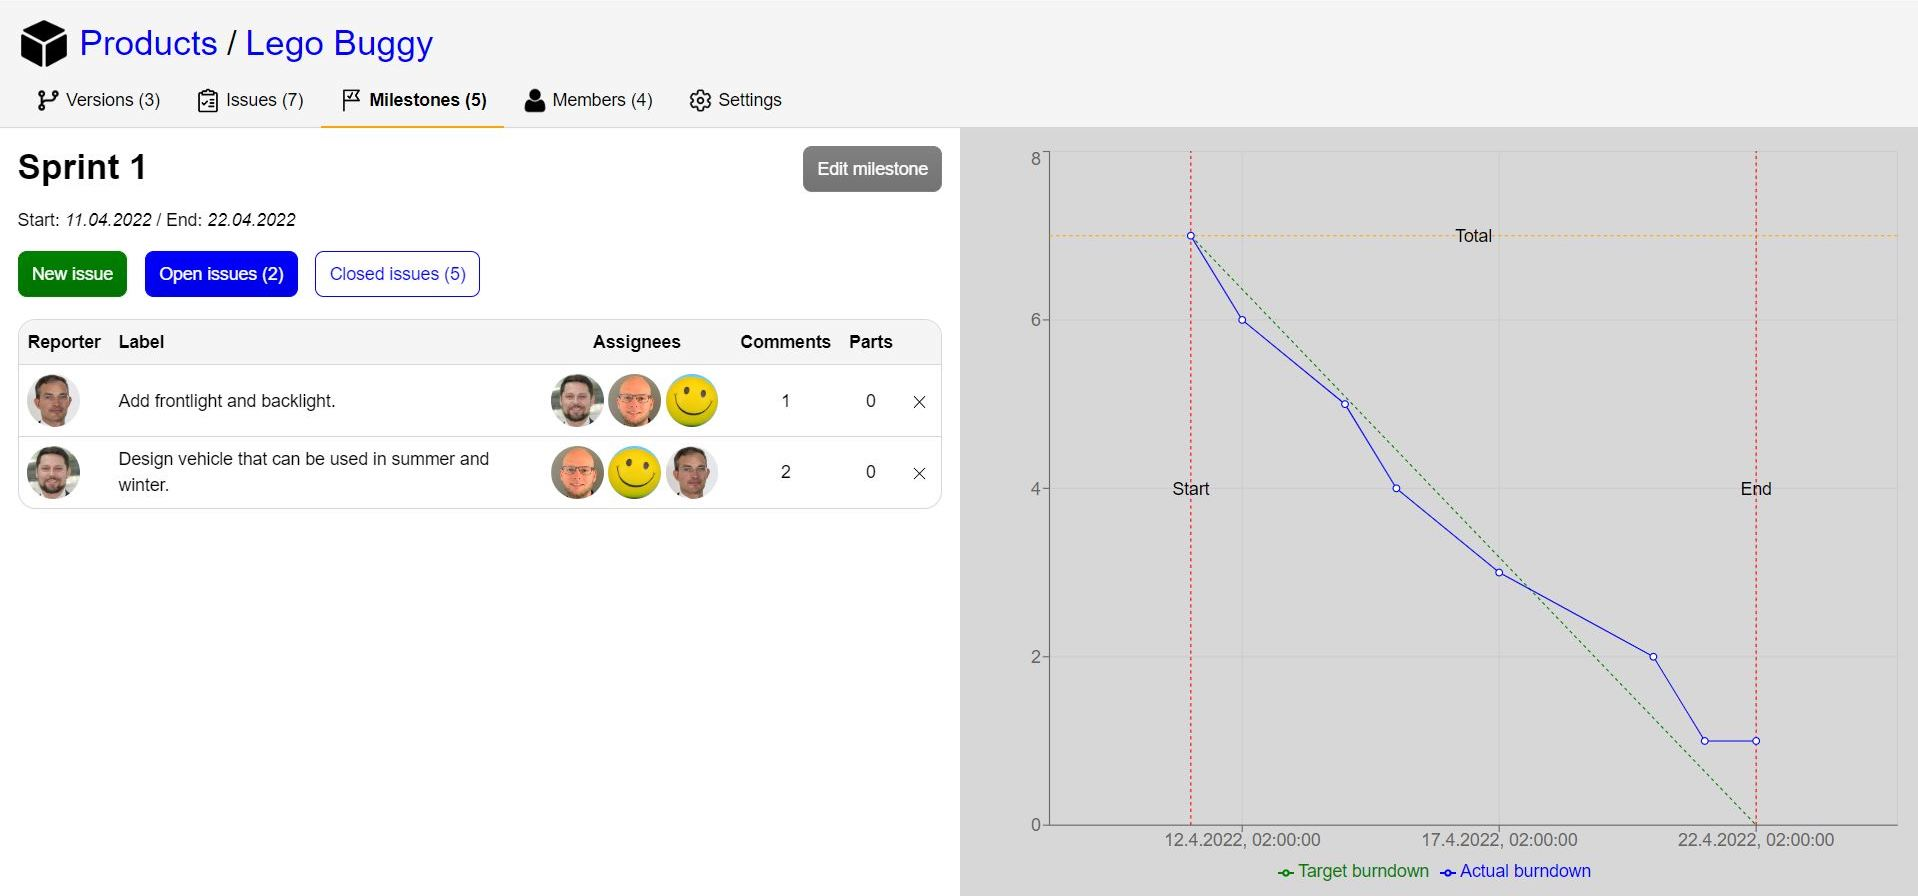
\includegraphics[width=0.5\textwidth]{sprintview.JPG}
    \caption{ProductMilestoneIssue view}
    \label{fig: sprintview}
\end{wrapfigure}

If a milestone is selected, a table with the attached issues is displayed [see Fig. \ref{fig: sprintview}]. This table is identical to the one in the ProductIssue view. Here you can also filter by open and closed issues. On the right side a burn down chart is displayed which shows the current progress of the milestone. The chart shows the start date, the end date, the number of issues and the progress until the current day. In the chart, the green line represents the target burndown and the blue graph the actual burndown. The target burndown distributes the open issues over the time span. The actual burndown drops by one for each issue that is closed.  Like in the ProductMilestone view, a click Edit Milestone button leads to the ProductMilestoneSettings view where the attributes of a milestone can be changed.

\subsubsection{ProductMember view}

\begin{wrapfigure}{r}{0.5\textwidth}
    \centering
    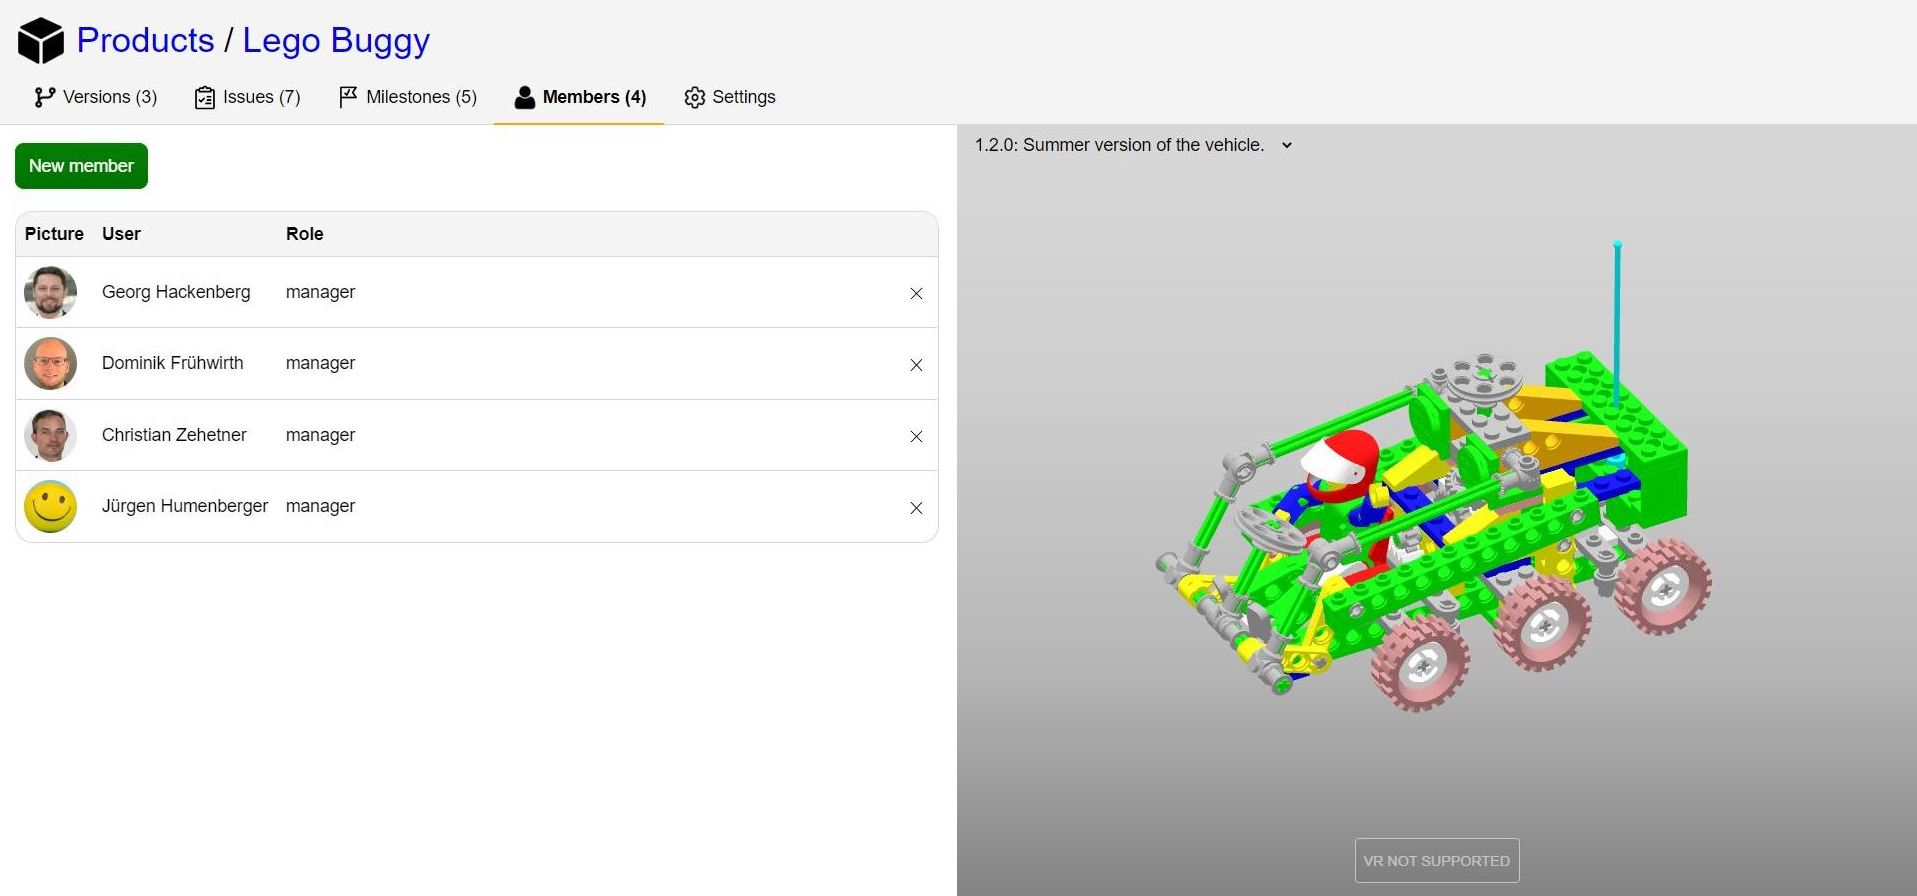
\includegraphics[width=0.5\textwidth]{memberview.JPG}
    \caption{Member view}
    \label{fig: memberview}
\end{wrapfigure}

To distribute the rights for a product, members are added to an existing product via the user interface. In the ProductMember view, a table shows all members who have access to the selected product [see Fig. \ref{fig: memberview}]. The table shows the user picture and the name of the user. The role column defines which rights the respective member has. At the moment there are three roles: \textit{manager, engineer, customer} as explained in the permission model.. As with every overview table, objects can be deleted from the list by clicking on the X button. The button New Member leads to the ProductMemberSettings view where new members can be added.